\newpage
\chapter[Cauchy's Integral Formula]{Cauchy's Integral Formula and its Applications}
\section{Cauchy's Integral Formula}
We have seen so far that if $f:\mathcal{R} \to \C$ is holomorphic on a starlit region $\mathcal{R}$ then
\[
\int_{\mathcal{C}} f = 0
\]
for any closed contour $\mathcal{C}$ in $\mathcal{R}$. What happens when $\mathcal{R}$ is not starlit?  

It may happen that while $\mathcal{R}$ itself is not starlit, the contour $\mathcal{C}$ is contained in a starlit subregion $\mathcal{S}$ of $\mathcal{R}$.

\begin{figure}[H]
\begin{tabular}{ccc}
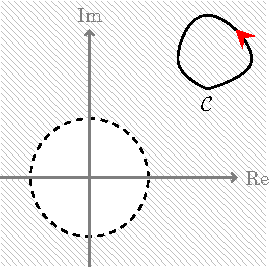
\includegraphics[scale=1]{ch5_notsc3} & \quad 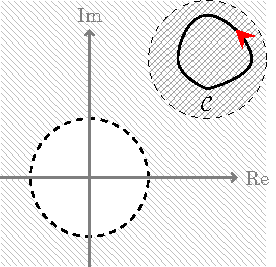
\includegraphics[scale=1]{ch5_notsc1} \quad & 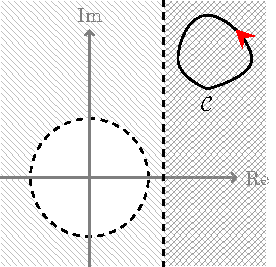
\includegraphics[scale=1]{ch5_notsc2}
\end{tabular}
\caption{The region $\mathcal{R}$ consists of the complex plane with a disc centred at the origin removed.  This region is not starlit, but there are starlit subregions of $\mathcal{R}$ containing the contour $\mathcal{C}$.}
\end{figure}

Thus if $f$ is holomorphic on $\mathcal{R}$, then $f$ is also holomorphic on $\mathcal{S}$ and so Cauchy's Theorem for Starlit Regions (Theorem~\ref{t:cauchyst}) gives
\[
\int_{\mathcal{C}} f=0.
\]

If $\mathcal{R}$ is not simply connected, then it may not be possible to do this; in particular, when $\mathcal{C}$ encloses a point $z_0$ at which $f$ is not holomorphic.  For example, suppose $f:\C \backslash \set{0} \to \C$ is defined by $f(z) = \dfrac{1}{z}$, and $\mathcal{C}$ is the contour shown in Figure~\ref{f:notsc}.  
\begin{figure}[H]
\centering
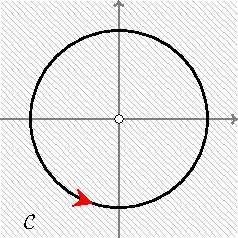
\includegraphics[scale=0.75]{ch5_notsc}
\caption{A contour $\mathcal{C}$ contained in the non-simply connected region $\C\backslash \set{0}$.}
\label{f:notsc}
\end{figure}

Here $\C \backslash \set{0}$ is not starlit, and there is no starlit subregion of $\C \backslash \set{0}$ containing $\mathcal{C}$.  Nonetheless, in certain circumstances, it is at least possible to replace $\mathcal{C}$ something easier in order to calculate the integral.

\begin{definition}
A contour $\mathcal{C}$, that is not closed, is said to be \emph{simple} if $\mathcal{C}$ does not intersect itself.  A \emph{simple closed contour $\mathcal{C}$} is one that does not intersect itself except that its start point is the same as its end point.
\end{definition}

\begin{figure}[H]
\centering
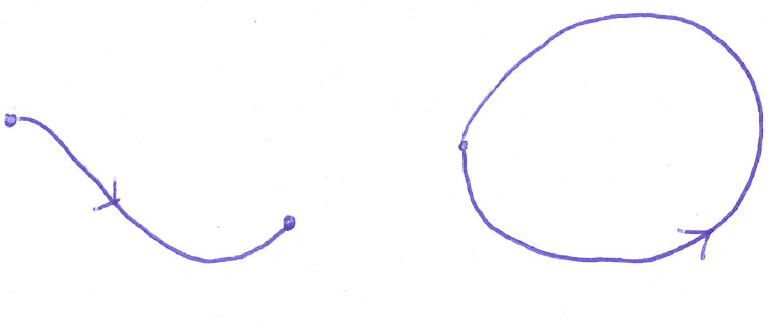
\includegraphics[scale=0.3]{ch5_simple_full}
\caption{Simple contours.}
\end{figure}
\begin{figure}[H]
\centering
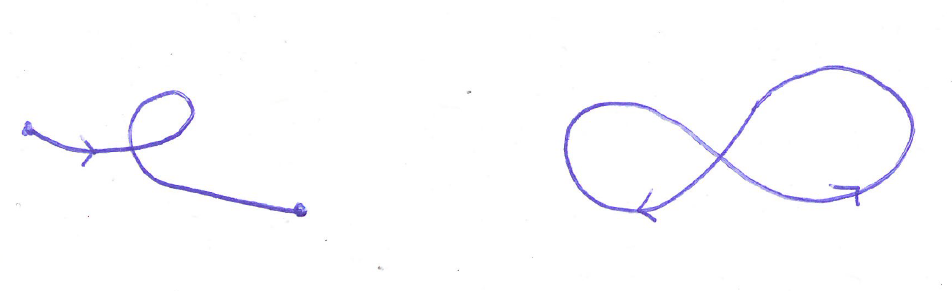
\includegraphics[scale=0.3]{ch5_nonsimple_full}
\caption{Non-simple contours.  Note that the closed, non-simple contour on the right has no obvious orientation - it is neither clockwise nor anticlockwise.}
\end{figure}


For a simple closed contour $\mathcal{C}$, when we speak of $\mathcal{C}$ being clockwise or anticlockwise, we mean relative to the points enclosed by $\mathcal{C}$.  In other words, a contour $\mathcal{C}$ is anticlockwise if, as we travel along $\mathcal{C}$, the region enclosed by $\mathcal{C}$ always lies to our left.  Again, we shall avoid giving a precise definition, and treat this notion informally.





The following Theorem shows us how in some cases, a potentially complicated contour integral may be reduced to an easier one.
\begin{theorem}[Shrinking Contour Theorem/Deformation Theorem]
\label{t:sc}
Let $\mathcal{R}$ be a simply connected region, $\mathcal{C}$ an anticlockwise, simple closed contour in $\mathcal{R}$, $z_0$ a point enclosed by $\mathcal{C}$ and $g$ a function which is holomorphic on $\mathcal{R} \backslash \set{z_0}$.  Then
\[
\int_{\mathcal{C}} g = \int_{\mathcal{C}_r} g
\]
where $\mathcal{C}_r$ is an anticlockwise circular contour with centre $z_0$ and radius $r$, which is small enough so that $\mathcal{C}_r$ is contained in $\mathcal{R}$.
\end{theorem}
\begin{center}
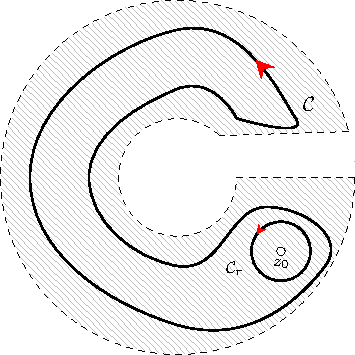
\includegraphics[scale=0.75]{ch5_scnotstarlit4}
\end{center}
{\bf Sketch of Proof}

Let us first consider the case where $\mathcal{R} = \C$ as shown:
\begin{center}
\altgraphics[scale=1]{ch5_shrinking_cont_full}{ch5_shrinking_cont}
\end{center}
\begin{blankbox}
Draw a straight line through $z_0$ to get two starlit subregions $\mathcal{R}_1$ and $\mathcal{R}_2$, with $g$ holomorphic on both $\mathcal{R}_1$ and $\mathcal{R}_2$. Join $\mathcal{C}$ and $\mathcal{C}_r$ along this straight line to get two new (simple, closed, anticlockwise) contours $\mathcal{C}_1$ and $\mathcal{C}_2$ contained in $\mathcal{R}_1$ and $\mathcal{R}_2$ respectively.

By Cauchy's Theorem for Starlit Regions,
\[
\int_{\mathcal{C}_1} g = \int_{\mathcal{C}_2} g = 0.
\]
Moreover,
\[
0= \int_{\mathcal{C}_1} f + \int_{\mathcal{C}_2} f = \int_{\mathcal{C}} f - \int_{\mathcal{C}_r} f,
\]
as the integrals along the straight line segments cancel, leaving us with
\begin{itemize}
\item an anticlockwise copy of $\mathcal{C}$, and
\item a clockwise copy of $\mathcal{C}_r$, i.e., the reverse of $\mathcal{C}_r$.
\end{itemize}
Thus
\[
\int_{\mathcal{C}} f = \int_{\mathcal{C}_r} f.
\]
\end{blankbox}

For more general simply connected regions $\mathcal{R}$, we may need to partition $\mathcal{R}$ into starlit subregions $\mathcal{R}_1,\mathcal{R}_2,\ldots, \mathcal{R}_n$, numbered so that $z_0 \in \mathcal{R}_n$. By joining points on $\mathcal{C}$, we get anticlockwise closed contours $\mathcal{C}^{(1)},\mathcal{C}^{(2)},\ldots,\mathcal{C}^{(n)}$, with $\mathcal{C}^{(j)}$ contained in $\mathcal{R}_j$ for each $j$.  Label the regions $\mathcal{R}_j$ so that $z_0 \in \mathcal{R}_n$. 

\begin{center}
\altgraphics[scale=0.3]{ch5_deformation1_full}{ch5_deformation2}
\end{center}

\begin{blankbox}
%\vspace*{12cm}
As before,
\[
\int_{\mathcal{C}} g = \int_{\mathcal{C}^{(1)}} g + \int_{\mathcal{C}^{(2)}} g + \ldots + \int_{\mathcal{C}^{(n)}} g,
\]
as the integrals along the connecting edges cancel in pairs.
\begin{comment}
\leftimage{
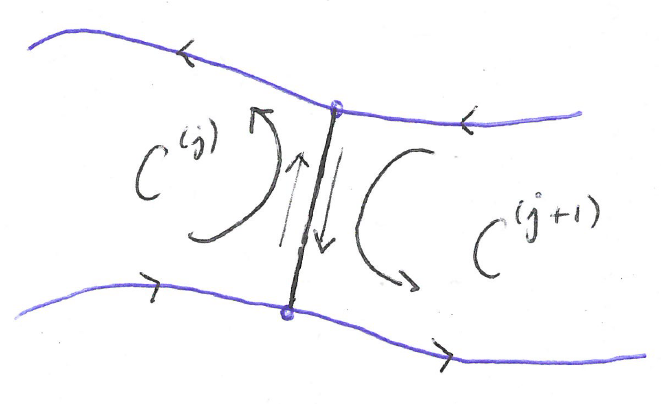
\includegraphics[scale=0.3]{ch5_deformation2_full}
}
{
The edge where $\mathcal{C}^{(j)}$ and $\mathcal{C}^{(j+1)}$ intersect is traversed in one direction along $\mathcal{C}^{(j)}$ and in the opposite direction along $\mathcal{C}^{(j+1)}$.  Thus when we compute the sum of the integral of $g$ along $\mathcal{C}^{(j)}$ and along $\mathcal{C}^{(j+1)}$, the contributions made by this connecting edge cancel.
}
\end{comment}

For each $j \neq n$, $g$ is holomorphic on $\mathcal{R}_j$, and $\mathcal{C}^{(j)}$ is a closed contour contained in the starlit region $\mathcal{R}_j$.  Thus by Cauchy's Theorem for Starlit regions, we have
\[
\int_{\mathcal{C}^{(j)}} g = 0\quad \text{ for } j=1,2,\ldots,n-1.
\]

Combining these two observations it follows that
\[
\int_{\mathcal{C}} g = \int_{\mathcal{C}^{(n)}} g,
\]
and thus we need to show that
\[
\int_{\mathcal{C}^{(n)}}g = \int_{\mathcal{C}_r} g.
\]
The proof of this is almost identical to the case $\mathcal{R}=\C$.
\end{blankbox}
\begin{comment}

While $\mathcal{R}_n$ is starlit, $\mathcal{R}_n \backslash \set{z_0}$ is not.  Thus we split $\mathcal{R}_n \backslash \set{z_0}$ into two starlit subregions, and construct contours $S_1$ and $S_2$ by connecting $\mathcal{C}^{(n)}$ and $\mathcal{C}_r$ as shown.
\begin{center}
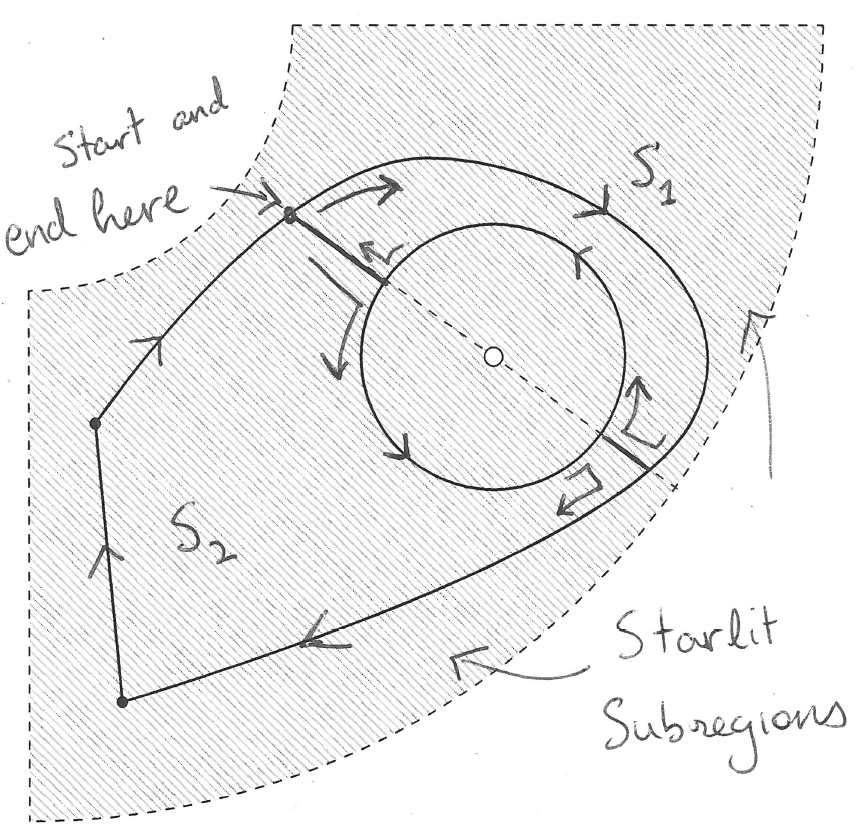
\includegraphics[scale=0.25]{ch5_shrinking}
\end{center}


By Cauchy's Theorem for Starlit Regions, we again have
\[
\int_{S_1} g = \int_{S_2} g = 0.
\]

Notice that if we join $S_1$ and $S_2$ we get a contour consisting of
\begin{itemize}
\item An anticlockwise copy of the circular contour $\mathcal{C}_r$, 
\item A clockwise copy of $\mathcal{C}^{(n)}$, i.e. the reverse of $\mathcal{C}^{(n)}$, and
\item two copies of each of the new edges connecting $\mathcal{C}^{(n)}$ and $\mathcal{C}_r$, one in each direction.
\end{itemize}
Thus we get
\[
\int_{S_1} g + \int_{S_2} g = \int_{\mathcal{C}_r} g - \int_{\mathcal{C}^{(n)}} g
\]
as the integrals along the new edges connecting $\mathcal{C}^{(n)}$ and $\mathcal{C}_r$ cancel, and we are left with $\mathcal{C}_r$ and the reverse of $\mathcal{C}^{(n)}$.
  
Hence
\[
0 = \int_{S_1} g + \int_{S_2} g = \int_{\mathcal{C}_r} g - \int_{\mathcal{C}^{(n)}} g
\]
and so
\[
\int_{\mathcal{C}_r} g = \int_{\mathcal{C}^{(n)}} g = \int_{\mathcal{C}} g.
\]
\blanksoff
%\vspace*{9cm}
\end{comment}

\qed

A very similar argument is used to prove Cauchy's Theorem for Simply Connected Regions.

\begin{theorem}[Cauchy's Theorem for Simply Connected Regions]
Let $f$ be a function that is holomorphic in a simply connected region $\mathcal{R}$, and let $\mathcal{C}$ be a closed contour in $\mathcal{R}$. Then
\[
\int_{\mathcal{C}} f = 0.
\]
\end{theorem}
{\bf Proof}
This is identical to the Proof of Theorem~\ref{t:sc}, except that now, $f$ is holomorphic on the starlit region $\mathcal{R}_n$, so that
\[
\int_{\mathcal{C}} f = \int_{\mathcal{C}_r} f =0.
\]
\qed


%\vspace*{7cm}





\begin{theorem}[Cauchy's Integral Formula]
\label{t:cauchyformula}
Let $\mathcal{R}$ be a simply connected region, $\mathcal{C}$ an anticlockwise simple closed contour in $\mathcal{R}$, $z_0$ a point enclosed by $\mathcal{C}$ and $f$ a function that is holomorphic on $\mathcal{R}$.  Then
\[
\int_{\mathcal{C}} \frac{f(z)}{z-z_0} \ dz = 2 \pi i f( z_0).
\]
\end{theorem}
\begin{proof}
Define a new function $g$ by the formula
\[
g(z) = \frac{f(z)}{z-z_0}
\]
so that $g$ is holomorphic on $\mathcal{R} \backslash \set{z_0}$, i.e., where $f$ is holomorphic and $z-z_0 \neq 0$.  Thus we are trying to show that
\[
\int_{\mathcal{C}} g = 2\pi i f(z_0).
\]
Using the Shrinking Contour Theorem~\ref{t:sc}, we may replace $\mathcal{C}$ with an anticlockwise circular contour $\mathcal{C}_r$ with centre $z_0$ and radius $r$ to get
\[
\int_{\mathcal{C}} g = \int_{\mathcal{C}_r} g
\]
whenever $r>0$ is small enough so that $\mathcal{C}_r$ is contained in $\mathcal{R}$.  

If we define $I$ by
\[
I = \left(\int_{\mathcal{C}_r} \frac{f(z)}{z-z_0}\ dz \right) - 2 \pi i f(z_0),
\]
then we want to show that $I=0$.  To do this, we will write $I$ as a single integral along $\mathcal{C}_r$ and use the Estimation Lemma (together with the fact that our definition of $I$ does not depend on our choice of sufficiently small $r$).

Parametrising $\mathcal{C}_r$ with $\gamma:[0,2\pi] \to \C$, $\gamma(t) = z_0 + r \exp (it)$, we have
\[
\int_{\mathcal{C}_r} \frac{1}{z-z_0}\ dz = \int_0^{2\pi} \frac{1}{z_0+r\exp(it)-z_0} \cdot i r\exp (it) \ dt = \int_0^{2\pi} i \ dt = 2 \pi i
\]
(which we saw in Exercise Sheet 2). Therefore, since $f(z_0)$ is a constant, we get
\[
2\pi i f(z_0) = \int_{\mathcal{C}_r} \frac{f(z_0)}{z-z_0}\ dz.
\]
Thus
\begin{align*}
I &= \int_{\mathcal{C}_r} \frac{f(z)}{z-z_0}\ dz - \int_{\mathcal{C}_r} \frac{f(z_0)}{z-z_0}\ dz \\
& = \int_{\mathcal{C}_r} \frac{f(z)-f(z_0)}{z-z_0}\ dz.
\end{align*}
To apply the Estimation Lemma, we need to find an upper bound for
\[
\abs{ \frac{f(z)-f(z_0)}{z-z_0} } \quad \text{ where } z \in \mathcal{C}_r.
\]
Since $\mathcal{C}_r$ is a circle with centre $z_0$ and radius $r$, it is clear that $\abs{z-z_0} = r$ for all $z \in \mathcal{C}_r$, and thus we look at $\abs{f(z)-f(z_0)}$.

Since $f$ is holomorphic on $\mathcal{R}$, it is continuous on $\mathcal{R}$ and in particular, continuous at $z_0$.  Thus given any $\epsilon>0$ there exists $\delta>0$ such that
\[
0 < \abs{z-z_0} < \delta \Rightarrow \abs{ f(z)-f(z_0) } < \epsilon.
\]
In other words, given any $\epsilon >0$, if we choose $r$ so that $0<r < \delta$, we have
\[
z \in \mathcal{C}_r \Rightarrow \abs{z-z_0} = r < \delta \Rightarrow \abs{f(z)-f(z_0)} < \epsilon.
\]
For any such $r$ we thus have
\[
z \in \mathcal{C}_r \Rightarrow \abs{\frac{f(z)-f(z_0)}{z-z_0}} = \frac{\abs{f(z)-f(z_0)}}{\abs{z-z_0}} < \frac{\epsilon}{r}.
\]
By the Estimation Lemma (using the fact that $\ell ( \mathcal{C}_r ) = 2 \pi r$), we see that
\[
\abs{\int_{\mathcal{C}_r} \frac{f(z)-f(z_0)}{z-z_0}\ dz} \leq \frac{\epsilon}{r} 2 \pi r = 2\pi \epsilon.
\]
However, since the definition of $I$ does not depend on our choice of (small) $r$, it follows that
\[
\abs{I} < 2 \pi \epsilon
\]
for all $\epsilon>0$.  Hence $\abs{I}=0$ which implies $I=0$, or in other words,
\[
\int_{\mathcal{C}} \frac{f(z)}{z-z_0}\ dz = 2 \pi i f(z_0).
\]
\end{proof}

\begin{note}
Cauchy's Integral Formula, and its proof, can be easily remembered using the following approximation: if $r$ is small and $z \in \mathcal{C}_r$ then $f(z) \approx f(z_0)$, hence
\[
\int_{\mathcal{C}_r} \frac{f(z)}{z-z_0}\ dz \approx \int_{\mathcal{C}_r} \frac{f(z_0)}{z-z_0}\ dz = f(z_0) \int_{\mathcal{C}_r} \frac{1}{z-z_0}\ dz = f(z_0) (2\pi i).
\]
\end{note}
Suppose we wish to evaluate the integral $\int_{\mathcal{C}} g$ of a continuous function $g$ along some closed contour $\mathcal{C}$.  If we can find some point $z_0$ enclosed by $\mathcal{C}$ and a function $f$ holomorphic on $\mathcal{R}$ with 
\[
g(z) = \frac{f(z)}{z-z_0} \quad \text{ for all }z \in \mathcal{C}
\]
then our integral may be evaluated using
\[
\int_{\mathcal{C}} g = \int_{\mathcal{C}} \frac{f(z)}{z-z_0}\ dz =  2\pi i f(z_0).
\]
In other words, it is enough to know the value of $f(z_0)$ in order to calculate $\int_{\mathcal{C}}g$.
\begin{example}
Evaluate the integral
\[
\int_{\mathcal{C}} \frac{\Log (z)}{z^2+9}
\]
where $\Log$ is the Principal Logarithm function and $\mathcal{C}$ is the anticlockwise circle with centre $4i$ and radius $3$.
\end{example}
%\vspace*{5cm}
\begin{solution}
We know that $\Log$ is holomorphic on $\C_{\pi}$, and moreover, we have
\[
z^2+9 = (z+3i)(z-3i).
\]
If we write
\[
\frac{\Log (z)}{z^2+9} = \frac{\Log (z)}{(z+3i)(z-3i)} = \frac{f(z)}{z-z_0}
\]
where $z_0=3i$ and
\[
f(z) = \frac{\Log (z)}{z+3i}
\]
then $z_0$ is enclosed by $\mathcal{C}$ and $f$ is holomorphic on $\C_{\pi} \backslash \set{-3i}$, which is a region containing $\mathcal{C}$.  However, it is clear that the region $\C_{\pi} \backslash \set{-3i}$ is not simply connected, so the hypotheses of Cauchy's Integral Formula are not fully satisfied.  We deal with this by replacing $\C_{\pi} \backslash \set{-3i}$ with a subregion that is simply connected.

\leftimage{
\altgraphics[scale=1]{ch5_cpi5}{ch5_cpi4}
}{
Indeed, if we consider the region $\mathcal{R} = \set{ z \in \C: \Im (z)>0}$, then we see that
\begin{itemize}
\item $\mathcal{R}$ is simply connected,
\item $f$ is holomorphic on $\mathcal{R}$, and
\item $\mathcal{C}$ is a simple, closed anticlockwise contour that is contained in $\mathcal{R}$ and encloses the point $z_0=3i$.
\end{itemize}
}




Therefore, we can apply Cauchy's Integral Formula, which gives
\begin{align*}
\int_{\mathcal{C}} \frac{\Log(z)}{z^2+9}\ dz &= \int_{\mathcal{C}} \frac{f(z)}{z-z_0}\ dz \\
& = 2 \pi i f(z_0) \\
& = 2 \pi i \left( \frac{\Log(3i)}{3i+3i} \right) \\
& = \frac{\pi}{6} \left( \log (3) + i \frac{\pi}{2} \right).
\end{align*}
\end{solution}
%\vspace*{5cm}



%\vspace*{8cm}

\begin{theorem}[Cauchy's Integral Formula for Derivatives; proof non examinable]
\label{t:cauchyd}
Let $\mathcal{R}$ be a simply connected region, $\mathcal{C}$ a simple, closed anticlockwise contour contained in $\mathcal{R}$ and $f$ a function that is holomorphic on $\mathcal{R}$. Then
\begin{enumerate}
\item $f$ is infinitely differentiable on $\mathcal{R}$, and
\item At every point $z$ in the region enclosed by $\mathcal{C}$, the $k^{th}$ derivative $f^{(k)}$ of $f$ satisfies
\[
f^{(k)}(z) = \frac{k!}{2\pi i} \int_{\mathcal{C}} \frac{f(\zeta)}{(\zeta-z)^{k+1}}\ d \zeta.
\]
\end{enumerate}
\end{theorem}

\begin{theorem}[Liouville's Theorem]
Let $f:\C \to \C$ be holomorphic (i.e. $f$ is holomorphic on the entire complex plane) and suppose that $f$ is bounded, i.e., there exists $M>0$ with $\abs{f(z)}\leq M$ for all $z \in \C$.  Then $f$ is constant.
\end{theorem}
{\bf Proof: } Exercise Sheet 4.

\section{Evaluating Real Integrals Using Cauchy's Integral Formula}
An important application of Cauchy's Integral Formula (Theorem~\ref{t:cauchyformula}) is that it allows us to evaluate certain \emph{real} integrals that would be difficult, if not impossible, to evaluate otherwise.  The following example illustrates the general method for doing so, which we shall develop in the next few sections.
\begin{example}
\label{e:realint1}
Let $R>1$, and define a contour $\cont_R$ by joining the line segment $[-R,R]$ and the upper semicircle $\mathcal{S}_R$ from $R$ to $-R$ via $iR$.  Use Cauchy's Integral Formula to evaluate
\[
\int_{\cont_R} \frac{1}{1+z^2}\ dz.
\]
\begin{center}
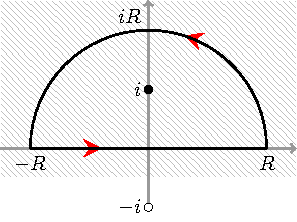
\includegraphics[scale=1.5]{ch5_cr1}
\end{center}
\end{example}
\begin{solution}
The function $f$ is holomorphic on $\C \backslash \set{i,-i}$.  Write
\[
\frac{1}{1+z^2} = \frac{1}{(z+i)(z-i)} = \frac{g(z)}{z-z_0}
\]
where
\[
g(z) = \frac{1}{z+i}\quad \text{ and } z_0=i.
\]
Then $g$ is holomorphic on $\C \backslash \set{-i}$ and in particular, on the simply connected region $\mathcal{R} = \set{ z \in \C: \Im (z) > - \frac{1}{2}}$.  Moreover, $\mathcal{C}_R$ is a closed, simple anticlockwise contour in $\mathcal{R}$ and $z_0=i$ is a point enclosed by $\mathcal{C}_R$.
\begin{comment}
\begin{center}
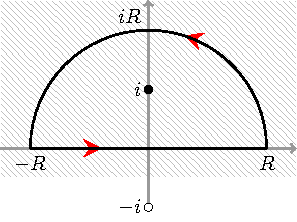
\includegraphics[scale=1]{ch5_cr1}
\end{center}
\end{comment}
Hence by Cauchy's Integral Formula,
\begin{align*}
\int_{\mathcal{C}_R} \frac{1}{1+z^2}\ dz &= \int_{\mathcal{C}_R} \frac{g(z)}{z-i}\ dz \\
&= 2 \pi i g(i) \\
& = 2\pi i \frac{1}{i+i} = \pi.
\end{align*}
(Note that  this integral does not depend on the value of $R$ once $R>1$).

\end{solution}

\begin{example}
Now, let's use Example~\ref{e:realint1} to evaluate the real integral
\[
\int_{-\infty}^{+\infty} \frac{1}{1+x^2}\ dx.
\]
\end{example}
\begin{solution}
Having evaluated the integral using Cauchy's Integral Formula, we now look at the integrals along the two paths $L_R$ and $S_R$;
\[
\int_{\mathcal{C}_R} \frac{1}{z^2+1}\ dz = \int_{L_R} \frac{1}{z^2+1}\ dz + \int_{S_R} \frac{1}{z^2+1}\ dz.
\]
parametrise $L_R$ with $\gamma_L:[-R,R] \to \C$, $\gamma(t)=t$, so that $\gamma'(t)=1$ and
\[
\int_{L_R} \frac{1}{1+z^2}\ dz = \int_{-R}^R \frac{1}{1+t^2}\ dt.
\]
We have seen already (Example~\ref{e:estimation}) that
\[
\lim_{R \to \infty} \int_{S_R} \frac{1}{1+z^2}\ dz = 0.
\]
Hence
\begin{align*}
\pi & = \lim_{R \to \infty} \int_{\mathcal{C}_R} \frac{1}{1+z^2}\ dz \\
& = \left( \lim_{R \to \infty} \int_{L_R} \frac{1}{1+z^2}\ dz \right) +  \left( \lim_{R \to \infty} \int_{S_R} \frac{1}{1+z^2}\ dz \right)  \\
& = \lim_{R \to \infty} \int_{-R}^R \frac{1}{1+t^2}\ dt + 0 \\
& = \int_{-\infty}^{\infty} \frac{1}{1+t^2}\ dt.
\end{align*}
So we have used contour integration to show that
\[
\int_{-\infty}^{\infty} \frac{1}{1+x^2}\ dx = \pi.
\]
\end{solution}


\begin{example}
\label{e:trig1}
We shall evaluate the integral
\[
\int_{\Gamma} \frac{2i}{3z^2-10z+3}\ dz,
\]
where $\Gamma$ is the anticlockwise unit circle $\set{z: \abs{z}=1}$, and use it to evaluate the real integral
\[
\int_0^{2\pi} \frac{1}{5-3\cos(t)}\ dt.
\]
\end{example}
\begin{solution}
If we factorise the denominator, we can write
\[
\frac{2i}{3z^2-10z+3} = \frac{2i}{(3z-1)(z-\frac{1}{3}}.
\]

The point $z_0=\frac{1}{3}$ is the only point enclosed by $\Gamma$ at which this function is not holomorphic.  If we let
\[
g(z) = \frac{2i}{3(z-3)}
\]
we have
\[
\frac{g(z)}{z-\frac{1}{3}} = \frac{2i}{(3z-1)(z-3)}
\]
and $g$ is holomorphic on the simply connected region $\set{z \in \C: \Re (z) < 2}$, which contains $\mathcal{C}$.  Thus
\begin{align*}
\int_{\Gamma} \frac{2i}{(3z-1)(z-3)}\ dz & = \int_{\Gamma} \frac{g(z)}{z-\frac{1}{3}}\ dz \\
& = 2\pi i g(\tfrac{1}{3}) \\
& = 2\pi i \left( - \frac{i}{4} \right) = \frac{\pi}{2}.
\end{align*}

For the second part, we parametrise $\Gamma$ using $\gamma:[0,2\pi]\to \C$, $\gamma(t)=e^{it}$ and use
\begin{align*}
\int_{\Gamma} f &= \int_0^{2\pi} f ( \gamma(t) ) \gamma'(t)\ dt \\
& = \int_0^{2\pi} \frac{2i}{3e^{2it}-10e^{it}+3}\cdot i e^{it}\ dt \\
& = \int_0^{2\pi} \frac{-2}{-10+3(e^{it}-e^{-it})}\ dt.
\end{align*}
Since $\cos(t) = \frac{1}{2}\brac{e^{it}-e^{-it}}$, it follows that
\[
\frac{-2}{-10+3(e^{it}+e^{-it})} = \frac{-2}{-10+6\cos(t)} = \frac{1}{5-3\cos(t)}.
\]
Hence
\[
\int_0^{2\pi} \frac{1}{5-3\cos(t)}\ dt = \int_{\Gamma} \frac{2i}{3z^2-10z+3} = \frac{\pi}{2}.
\]
\end{solution}


We can generalise the method of Example~\ref{e:trig1} to evaluate other real trigonometric integrals.
\begin{definition}
A \emph{Rational Function} $R:U \to \R$, where $U \subseteq \R^2$, is a function of the form
\[
R(x,y) = \frac{f(x,y)}{g(x,y)},
\]
where $f,g: \mathbb{R}^2 \to \R$ are two polynomials in $x$ and $y$ with real coefficients.
\end{definition}
We will now describe how to use contour integration to evaluate integrals of the form
\[
\int_0^{2\pi} R( \cos (t), \sin (t) )\ dt,
\]
where $R$ is a rational function of two real variables. For example, if $R$ is defined by
$
\displaystyle R(x,y) = \frac{1}{16x^2+25y^2},
$
then we are looking at the integral
\[
\int_0^{2\pi} R(\cos (t) , \sin (t) )\ dt = \int_0^{2\pi} \frac{1}{16 \left( \cos (t) \right)^2+25 \left( \sin (t) \right)^2}\ dt.
\]
Note that $\cos$ and $\sin$ are periodic with period $2\pi$, and that the above integral has limits $0$ and $2\pi$.

\begin{example}
\label{e:trig2}
For any rational function $R$ of two real variables, with $R(\cos(t),\sin(t))$ defined for every $t \in [0,2\pi]$, we can find a suitable closed contour $\mathcal{C}$ and complex function $f$ so that
\[
\int_0^{2\pi} R ( \cos(t), \sin (t) ) = \int_{\mathcal{C}} f.
\]
\begin{blankbox}
Let $\mathcal{C}$ be the anticlockwise circle $\set{z \in \C: \abs{z}=1}$, parametrised using $\gamma:[0,2\pi] \to \C,\ \gamma(t) = \exp(it)$. Let $f$ denote the complex function we are looking for, so we want
\[
\int_0^{2\pi} R ( \cos(t),\sin(t) ) \ dt = \int_{\mathcal{C}} f = \int_0^{2\pi} f \left( \gamma (t) \right) \gamma' (t)\ dt,
\]
or in other words,
\begin{equation}
\tag{R1}\label{e:r1}
f( \gamma(t) ) = \frac{1}{\gamma'(t)} \cdot R( \cos(t), \sin (t) ).
\end{equation}
For each $z \in \mathcal{C}$, $z= \exp(it)$ for some $t \in [0,2\pi]$ and so
\begin{align*}
\cos(t) & = \frac{\exp(it)+\exp(-it)}{2}  = \frac{z+z^{-1}}{2} \\
\sin(t) & = \frac{\exp(it)-\exp(-it)}{2i} =  \frac{z-z^{-1}}{2i} \\
\end{align*}
Hence for $z=\exp (it) \in \mathcal{C}$, we have
\begin{equation}
\tag{R2}\label{e:r2}
 R ( \cos (t), \sin (t) )  = R \left( \frac{z+z^{-1}}{2}, \frac{z-z^{-1}}{2i} \right), 
 \end{equation}
(this is not true for all $z$, only for $z$ lying on the contour $\mathcal{C}$). Moreover, $\gamma'(t) = i \exp (it) = iz$; so combining~\eqref{e:r1} and~\eqref{e:r2}, we define
\[
f(z) = R \left( \frac{z+z^{-1}}{2}, \frac{z-z^{-1}}{2i} \right) \cdot \frac{1}{iz}.
\]
Then
\begin{align*}
\int_{\mathcal{C}} f & = \int_0^{2\pi} f( \gamma(t)) \gamma'(t) \\
& = \int_0^{2\pi} R \left( \tfrac{1}{2}(\exp(it)+\exp(-it)),\tfrac{1}{2i}(\exp(it)-\exp(-it)) \right) \cdot \frac{1}{i\exp(it)} \cdot i\exp(it)\ dt \\
&= \int_0^{2\pi} R( \cos (t) , \sin (t))\ dt.
\end{align*}
\end{blankbox}
\end{example}
\begin{example}
Use a suitable contour integral to evaluate
\[
\int_0^{2\pi} \frac{1}{2+\sin \theta}\ d \theta.
\]
\begin{solution}
With $\mathcal{C}$ the anticlockwise unit circle, we have
\begin{align*}
\int_0^{2\pi} \frac{1}{2+\sin \theta}\ d \theta & = \int_{\mathcal{C}} \frac{1}{2+\frac{z-z^{-1}}{2i}} \cdot \frac{1}{iz}\ dz \\
& = \int_{\mathcal{C}} \frac{2}{z^2+4iz-1}\ dz \\
& = \int_{\mathcal{C}} \frac{2}{(z-(-2+\sqrt{3})i)(z-(-2-\sqrt{3})i)}\ dz.
\end{align*}
By Cauchy's Integral Formula, this integral has the value
\[
2\pi i \cdot \frac{2}{(-2+\sqrt{3})i-(-2-\sqrt{3})i} = \frac{2\pi}{\sqrt{3}}.
\]
\end{solution}
\end{example}

\begin{example}
Set up a contour integral that could be used to evaluate
\[
\int_0^{2\pi} \frac{1}{16 \cos^2 (t) + 25 \sin^2 (t)}\ dt.
\]
\begin{solution}
Here $R(x,y) = \dfrac{1}{16x^2+25y^2}$, so the required integral (with $\mathcal{C}$ the anticlockwise circle $\set{z \in \C : \abs{z}=1 }$) is
\begin{align*}
\int_{\mathcal{C}} R \left( \frac{z+z^{-1}}{2}, \frac{z-z^{-1}}{2i} \right) \cdot \frac{1}{iz}\ dz & = \int_{\mathcal{C}} \frac{1}{16\left(\frac{1}{2}(z+z^{-1})\right)^2+25\left(\frac{1}{2i}(z-z^{-1}) \right)^2} \cdot \frac{1}{iz}\ dz \\
& = \int_{\mathcal{C}} \frac{1}{4(z+2+z^{-2})-\frac{25}{4}(z^2-2+z^{-2})} \cdot \frac{1}{iz}\ dz \\
& = \int_{\mathcal{C}} \frac{4i}{9z^4-82z^2+9}\ dz.
\end{align*}
We do not yet know how to evaluate this integral, we shall do this in Chapter 6.
\end{solution}
\end{example}


\section{Series Representations of Holomorphic Functions}
\begin{definition}
A sequence $z_n$ of complex numbers is said to converge to a complex number $z$ if, for all $\epsilon>0$ there is a natural number $N$ such that $n \geq N$ implies that $\abs{z_n-z}<\epsilon$.

An infinite series $\sum_{k=1}^{\infty} a_k$ is said to converge to a complex number $s$ if the sequence of partial sums $s_n:= \sum_{k=1}^n a_k$ converges to $s$.  When this occurs we write $\sum_{k=1}^{\infty} a_k = s$.
\end{definition}

For a fixed $z_0 \in \C$, a \emph{power series} (centred at $z_0$) is a series of the form $\displaystyle \sum_{n=0}^{\infty} a_n (z-z_0)^n$, where $a_n$ are complex numbers.  As with power series in $\mathbb{R}$, a complex power series may converge for some values of $z$ and diverge for others.  Note that if $\mathcal{S}$ denotes the subset
\[
\mathcal{S} = \set{ z \in \C: \sum_{n=0}^{\infty} a_n(z-z_0)^n \text{ converges } },
\]
then we get a function $f:\mathcal{S} \to \C$ defined by
\[
f(z) = \sum_{n=0}^{\infty} a_n (z-z_0)^n.
\]


\begin{theorem}[Taylor's Theorem]
\label{t:taylor}
Let $\mathcal{R}$ be a region, $f:\mathcal{R} \to \C$ holomorphic and $z_0$ a point in $\mathcal{R}$.  Then $f$ can be represented by the power series
\[
f(z) = \sum_{n=0}^{\infty} \frac{f^{(n)}(z_0)}{n!} (z-z_0)^n
\]
for all $z \in D(z_0;R)$, whenever $R>0$ is small enough so that $D(z_0;R) \subseteq \mathcal{R}$.
\end{theorem}
\begin{center}
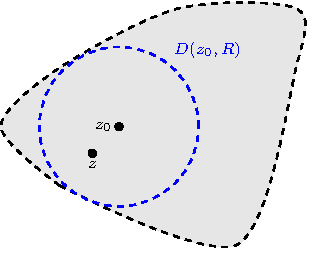
\includegraphics[scale=1]{ch5_taylordisc_full}
\end{center}
Before proving Taylor's Theorem, we need the following lemma:
\begin{lemma}
\label{l:taylor}
Let $f:\mathcal{R} \to \C$ be a function, $z_0 \in \mathcal{R}$ and $R>0$ be such that $D(z_0,R) \subseteq \mathcal{R}$.  Then for any $0<r<R$, $z \in D(z_0,r)$ and $\zeta \in \mathcal{C}_r$ we have
\[
\frac{f(\zeta)}{\zeta-z} = \left( \sum_{j=0}^n \frac{(z-z_0)^jf(\zeta)}{(\zeta-z_0)^{j+1}} \right) + \frac{(z-z_0)^{n+1} f ( \zeta)}{(\zeta-z_0)^{n+1}(\zeta-z)},
\]
where $\mathcal{C}_r$ is the anticlockwise circular contour with centre $z_0$ and radius $r$.
\begin{center}
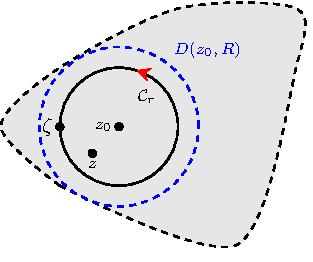
\includegraphics[scale=1]{ch5_taylordisclemma}
\end{center}
\end{lemma}

\begin{proof}
Note that we can write
\begin{equation}
\label{e:taylor1}\tag{T1}
\frac{1}{\zeta-z} = \frac{1}{\zeta-z_0}\cdot \frac{1}{\brac{1-\frac{z-z_0}{\zeta-z_0}}}.
\end{equation}
Rearranging the formula for a finite geometric sum,
\[
\sum_{j=0}^n w^j = \left( \frac{1-w^{n+1}}{1-w} \right),\quad\text{gives}\quad \frac{1}{1-w} = \left( \sum_{j=0}^n w^j \right) + \frac{w^{n+1}}{1-w},
\]

and so substituting $w = \dfrac{z-z_0}{\zeta-z_0}$ we get
\begin{align*}
\frac{1}{\brac{1-\frac{z-z_0}{\zeta-z_0}}} & = \left(\sum_{j=0}^n \left(\frac{z-z_0}{\zeta-z_0}\right)^j \right) + \frac{(z-z_0)^{n+1}}{\brac{\zeta-z_0}^{n+1}\brac{1-\frac{z-z_0}{\zeta-z_0}}} \\
& = \left(\sum_{j=0}^n \left(\frac{z-z_0}{\zeta-z_0}\right)^j \right) + \frac{\brac{z-z_0}^{n+1}}{\brac{\zeta-z_0}^n \brac{\zeta-z}}.
\end{align*}
Combining this with~\eqref{e:taylor1}, and multiplying both sides by $f(\zeta)$ we get
\[
\frac{f(\zeta)}{\zeta-z} = \left( \sum_{j=0}^n (z-z_0)^j \frac{f(\zeta)}{(\zeta-z_0)^{j+1}} \right) + \frac{\brac{z-z_0}^{n+1}f(\zeta)}{\brac{\zeta-z_0}^{n+1} \brac{\zeta-z}}
\]
\end{proof}

\begin{exercise}
Use the following steps to prove this Theorem (for now, you should assume the result of Lemma~\ref{l:taylor}).  Fix $r$ with $0<r<R$ and let $\mathcal{C}_r$ be the anticlockwise circular contour with centre $z_0$ and radius $R$.
\begin{enumerate}
\item[(i)]  Explain why 
\[
f(z) = \frac{1}{2\pi i} \int_{\mathcal{C}_r} \frac{f(\zeta)}{\zeta-z}\ d\zeta
\]
for all $z \in D(z_0,r)$.

\item[(ii)] Use Lemma~\ref{l:taylor} to show that
\[
2\pi i f( z) = \left( \sum_{j=0}^n (z-z_0)^j  \int_{\mathcal{C}_r} \frac{f(\zeta)}{(\zeta-z_0)^{j+1}}\ d\zeta \right) + \int_{\mathcal{C}_r} \frac{\brac{z-z_0}^{n+1}f(\zeta)}{\brac{\zeta-z_0}^{n+1} \brac{\zeta-z}}\ d\zeta
\]

\item[(iii)] Use Cauchy's Integral Formula for Derivatives to show that
\[
f(z) = f(z_0)+(z-z_0)f'(z_0)+\frac{(z-z_0)^2f''(z_0)}{2!}+\ldots+ \frac{(z-z_0)^n f^{(n)}(z_0)}{n!} + I_n,
\]
where $I_n = \displaystyle \frac{1}{2\pi i}\int_{\mathcal{C}_r}  \frac{\brac{z-z_0}^{n+1}f(\zeta)}{\brac{\zeta-z_0}^{n+1} \brac{\zeta-z}}\ d\zeta.$.
\item[(iv)] Show that
\begin{itemize}
\item $\abs{\zeta-z} \geq r - \abs{z-z_0}$ for all $\zeta \in \mathcal{C}_r$ and $z \in D(z_0,r)$, and that
\item there exists $K \geq 0$ with $\abs{f(\zeta)} \leq K$ for all $\zeta \in \mathcal{C}_r$.
\end{itemize}
\item[(v)] Use part (iv) and the Estimation Lemma to show that
\[
\abs{I_n} \leq \frac{1}{2\pi} \cdot \abs{\frac{z-z_0}{\zeta-z_0}}^{n+1} \cdot \frac{K}{r-\abs{z-z_0}}
\]
\item[(vi) ] Use part (v) to show that $\abs{I_n} \to 0$ and $n \to \infty$, and explain why this completes the proof.
\end{enumerate}
\end{exercise}

\begin{proof}[of Taylor's Theorem~\ref{t:taylor}]
Choose $r>0$ with $0 < r < R$ and let $\mathcal{C}_r$ be the anticlockwise circle with centre $z_0$ and radius $r$.  Then by Cauchy's Integral Formula,
\[
f(z) = \frac{1}{2\pi i} \int_{\mathcal{C}_r} \frac{f(\zeta)}{\zeta-z}\ d\zeta
\]
for all $z$ with $\abs{z-z_0}<r$.
\begin{center}
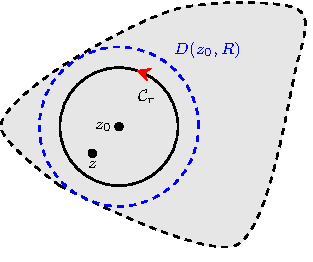
\includegraphics[scale=1]{ch5_taylordiscproof_full}
\end{center}

Together with Lemma~\ref{l:taylor} we see that
\[
2\pi i f(z) = \int_{\mathcal{C}_r} \left[ \left( \sum_{j=0}^n (z-z_0)^j \frac{f(\zeta)}{(\zeta-z_0)^{j+1}} \right) + \frac{\brac{z-z_0}^{n+1}f(\zeta)}{\brac{\zeta-z_0}^{n+1} \brac{\zeta-z}}  \right]\ d \zeta. 
\]
Using linearity of contour integrals, we first get
\[
2\pi i f(z) = \left( \sum_{j=0}^n \int_{\mathcal{C}_r} (z-z_0)^j \frac{f(\zeta)}{(\zeta-z_0)^{j+1}}\ d\zeta \right) + \int_{\mathcal{C}_r} \frac{\brac{z-z_0}^{n+1}f(\zeta)}{\brac{\zeta-z_0}^{n+1} \brac{\zeta-z}}\ d\zeta.
\]
and noting that since we are integrating with respect to $\zeta$, the $(z-z_0)$ terms are constant, this becomes
\[
2\pi i f( z) = \left( \sum_{j=0}^n (z-z_0)^j  \int_{\mathcal{C}_r} \frac{f(\zeta)}{(\zeta-z_0)^{j+1}}\ d\zeta \right) + \int_{\mathcal{C}_r} \frac{\brac{z-z_0}^{n+1}f(\zeta)}{\brac{\zeta-z_0}^{n+1} \brac{\zeta-z}}\ d\zeta
\]
(we leave the last term as it is for now).

Using Cauchy's Integral Formula For Derivatives (Theorem~\ref{t:cauchyd}), and dividing both sides by $2\pi i$, this becomes
\[
f(z) = f(z_0)+(z-z_0)f'(z_0)+\frac{(z-z_0)^2f''(z_0)}{2!}+\ldots+ \frac{(z-z_0)^n f^{(n)}(z_0)}{n!} + I_n,
\]
where 
\[
I_n = \frac{1}{2\pi i}\int_{\mathcal{C}_r}  \frac{\brac{z-z_0}^{n+1}f(\zeta)}{\brac{\zeta-z_0}^{n+1} \brac{\zeta-z}}\ d\zeta.
\]
To complete the proof, we must show that $I_n \to 0$ as $n \to \infty$.  We shall use the Estimation Lemma to do this.

\begin{itemize}
\item For $\zeta \in \mathcal{C}_r$, we have $\abs{\zeta-z_0}=r$, and since $z$ is enclosed by $\mathcal{C}_r$, $\abs{z-z_0}<r$.
\item Since $f$ is continuous on $\mathcal{C}_r$, there is some real number $K \geq 0$ such that $\abs{f(\zeta)} \leq K$ for all $\zeta$ in $\mathcal{C}_r$.  To see this, note that if $\mathcal{C}_r$ is parametrised by the continuous function $\gamma:[0,2\pi] \to \C$, $\gamma (t) = z_0+r e^{it}$, then $t \mapsto \abs{f(\gamma(t))}$ is a continuous, real-valued function on a closed interval, hence is bounded by the Extreme Value Theorem.
\item By the backwards triangle inequality,
\[
\abs{\zeta-z} = \abs{\zeta-z_0+z_0-z} \geq \abs{\abs{\zeta-z_0}-\abs{z_0-z}} = r - \abs{z_0-z},
\]
a strictly positive constant since $z$ is fixed and $\abs{z_0-z}<r$.
\end{itemize}
Hence for all $\zeta \in \mathcal{C}_r$ we have
\[
\abs{\frac{\brac{z-z_0}^{n+1}f(\zeta)}{\brac{\zeta-z_0}^{n+1} \brac{\zeta-z}} } = \abs{\frac{z-z_0}{\zeta-z_0}}^{n+1}\cdot \frac{\abs{f(\zeta)}}{\abs{\zeta-z}} \leq \abs{\frac{z-z_0}{\zeta-z_0}}^{n+1} \cdot \frac{K}{r-\abs{z-z_0}}
\]
Thus by the Estimation Lemma,
\[
\abs{I_n} = \abs{\frac{1}{2\pi i}\int_{\mathcal{C}_r}  \frac{\brac{z-z_0}^{n+1}f(\zeta)}{\brac{\zeta-z_0}^{n+1} \brac{\zeta-z}}\ d\zeta} \leq \frac{1}{2\pi} \cdot \abs{\frac{z-z_0}{\zeta-z_0}}^{n+1} \cdot \frac{K}{r-\abs{z-z_0}},
\]
Since $\abs{z-z_0}<\abs{\zeta-z_0}$, $\abs{\dfrac{z-z_0}{\zeta-z_0}}<1$ and so
$\displaystyle \abs{\frac{z-z_0}{\zeta-z_0}}^{n+1} \to 0 $ as  $n \to \infty$.

Since all other terms in the estimate are constant, this shows that $I_n \to 0$ as $n \to \infty$.

\end{proof}

Many familiar examples of Taylor Series from the real case are also valid for the corresponding complex functions:
\begin{center}
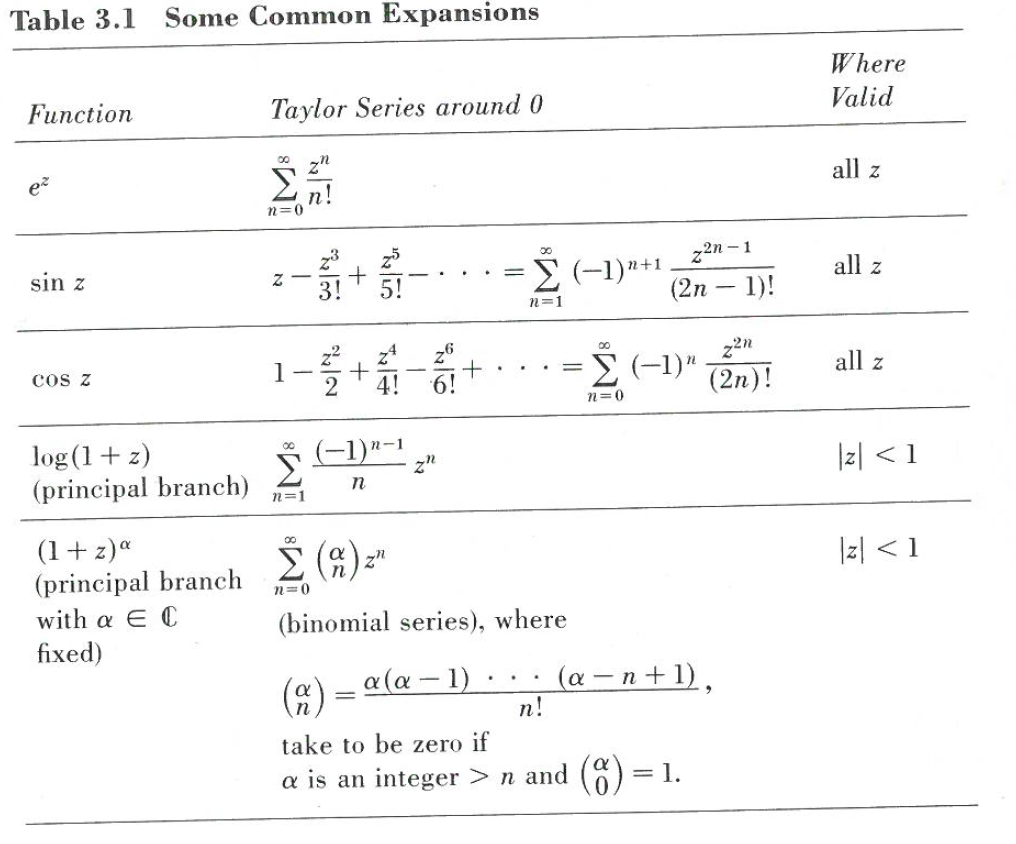
\includegraphics[scale=0.5]{ch5_taylor_examples}
\end{center}
These examples can be computed in exactly the same way as the corresponding real series.  In fact, we could say a lot more about complex Taylor Series, but we will not have time to do so in this module. 
\begin{example}
The Taylor Series expansion of a function $f:\mathcal{R} \to \C$ at a point $z_0 \in \mathcal{R}$ may not be valid everywhere in the domain of $f$.  For example, let us examine the Taylor series at $z=0$ of the function $f:\C \backslash \set{-i,i} \to \C$ defined by
\[
f(z) = \frac{1}{1+z^2}.
\]
\end{example} 
\begin{blankbox}
This function is holomorphic on $\C \backslash \set{-i,i}$, and by differentiation we can show that its Taylor series at $z=0$ is
\[
\sum_{n=0}^{\infty} (-1)^{n} z^{2n}.
\]
The largest disc centred at $0$ that is contained in $\C \backslash \set{-i,i}$ is $D(0,1)$, hence this Taylor Series is valid (i.e. converges to $f(z)$) at every point of this disc by Theorem~\ref{t:taylor}.  However, Theorem~\ref{t:taylor} tells us nothing about convergence of this series at points of $\C \backslash \set{-i,i}$ that lie outside of this disc (in fact the series diverges at these points).
\begin{center}
\begin{tabular}{cc}
\altgraphics[scale=1]{ch5_taylorexample2_full}{ch5_taylorexample2} & \altgraphics[scale=1]{ch5_taylorexample3_full}{ch5_taylorexample3}
\end{tabular}
\end{center}

Similarly, if we compute the Taylor Series for $f$ at $z=2+i$ (which we won't do, but we know it exists), Theorem~\ref{t:taylor} tells us that this series converges for all $z$ inside the disc $D(2+i,2)$.
\end{blankbox}



\begin{remark}
It is worth pointing out some of the differences between the real and complex versions of Taylor's Theorem.
\begin{enumerate}
\item[(i)]  In the complex case, once we know that $f$ is differentiable everywhere on an open set $\mathcal{R}$ (i.e. holomorphic on $\mathcal{R}$), we know that $f$ can be represented by a Taylor series.  For real functions it is not enough to know that $f$ is differentiable on an open interval; $f$ must be infinitely differentiable.
\item[(ii)] There are examples of real functions that are infinitely differentiable, but whose Taylor series have radius on convergence $0$, e.g., the function $f$ defined by $f(x) = e^{-1/x^2}$ for $x \neq 0$ and $f(0)=0$.  This cannot happen in the complex case; the radius of convergence is always positive.
\end{enumerate}
\end{remark}